\documentclass[11pt,a4paper]{article}
\usepackage[utf8]{inputenc}
\usepackage[T1]{fontenc}
\usepackage[french]{babel}
\usepackage[margin=1.8cm]{geometry}
\usepackage{graphicx}
\usepackage{hyperref}
\usepackage{enumitem}
\usepackage{titlesec}

\setlist{nosep,leftmargin=1.2em}
\titlespacing*{\section}{0pt}{0.4em}{0.2em}
\titleformat{\section}{\normalfont\bfseries\large}{\thesection}{0.5em}{}
\setlength{\parskip}{0.2em}
\setlength{\parindent}{0pt}

\title{\vspace{-1.5cm}Rapport individuel --- It\'eration 2}
\author{Alexis Briend (\texttt{abd7852}) --- Projet Long SHDL}
\date{11 mai 2026}

\begin{document}
\maketitle
\vspace{-2em}

\section*{Contexte}
Responsable de la \textbf{structure g\'en\'erale} et de l'\textbf{interpr\'etation du SHDL} (\textsc{Scrum-23}). Objectif sprint~2~: remplacer le parser \`a descente r\'ecursive du sprint~1 par une version \emph{LL(1) table-driven} stricte, et brancher concr\`etement parser et simulateur via une couche de conversion. Atteint sur 82~commits.

\section*{Activit\'es r\'ealis\'ees}
\begin{itemize}
  \item \textbf{Parser LL(1) table-driven} (\texttt{parser/ll1/tabledriven/})~: table $M[NT,T]$ b\^atie depuis \textsc{First}/\textsc{Follow} (\texttt{TableBuilder}, lookup $O(1)$), driver \`a pile g\'en\'erique sans \emph{switch} (\texttt{CstParser}). Grammaire gel\'ee par \texttt{GrammarFreezeTest}, sans conflit \textsc{First}/\textsc{First} ni \textsc{First}/\textsc{Follow}.
  \item \textbf{Concrete Syntax Tree} en remplacement de l'AST~: types \texttt{sealed} \texttt{CstNode = CstLeaf | CstInternal} (records immuables), navigation \texttt{first}/\texttt{allOf}/\texttt{has}, offsets pr\'eserv\'es, trivia filtr\'es.
  \item \textbf{Conversion CST $\to$ \texttt{simulateur.Module}} (\texttt{parser/conversion/}, spec \texttt{docs/specs/2026-05-06-cst-conversion-design.md})~: combinatoire scalaire stricte. Hors-scope (vecteurs, m\'emoire, appel de module, doublons) rejet\'es par \texttt{ConversionException} typ\'ee avec offset.
  \item \textbf{Bug fix amont}~: \texttt{simulateur.Erwan.OR()} retournait \texttt{Op.AND}, corrig\'e avec test sentinelle anti-r\'egression.
\end{itemize}

\section*{R\'esultats}
\begin{itemize}
  \item \textbf{193 tests JUnit verts} (+86 vs sprint~1) sur 39~classes~: parser (offsets, $\varepsilon$-productions, erreurs avec position), conversion (cas nominaux \texttt{ET}/\texttt{OU}/\texttt{NOT}, rejets exhaustifs), bout-en-bout (\texttt{xor} via \texttt{FileSimulateur}).
  \item \textbf{14 fichiers Java} ajout\'es, int\'egration r\'eussie avec Erwan (\texttt{parser/lexer/}) et Mati (\texttt{simulateur.Module}, \texttt{FileSimulateur}).
\end{itemize}

\begin{center}
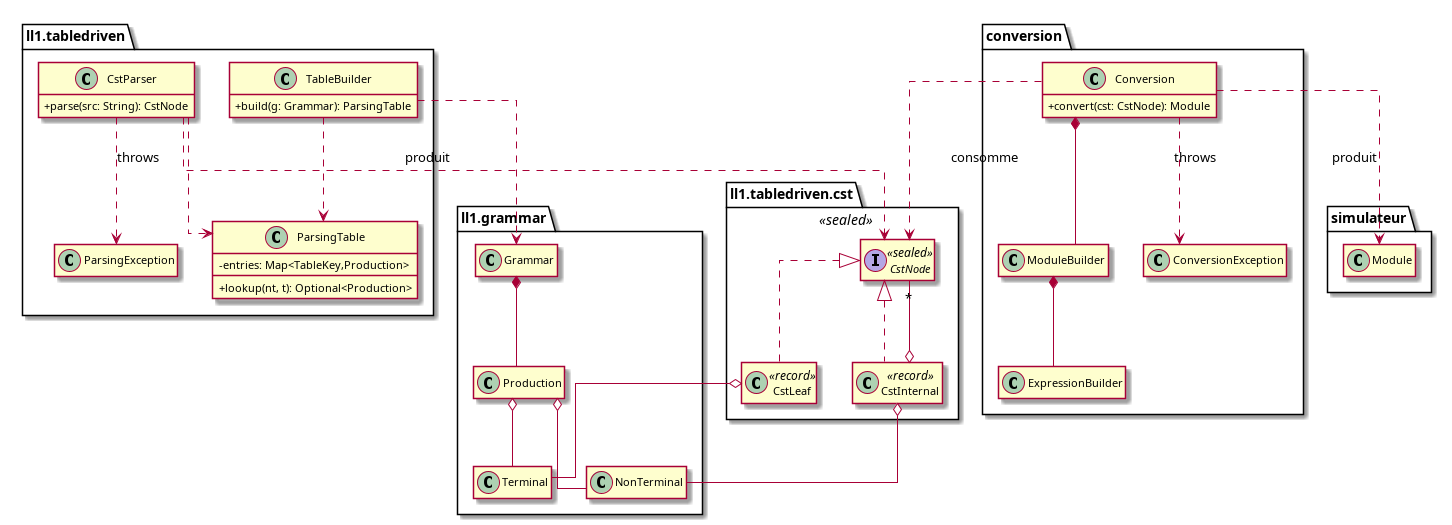
\includegraphics[width=0.95\textwidth]{cst-classes.png}\\
{\small Figure --- Cha\^ine parser $\to$ CST $\to$ conversion $\to$ \texttt{simulateur.Module} (source \texttt{cst-classes.puml}).}
\end{center}

\section*{Difficult\'es et r\'eussites}
Difficult\'e~: \emph{instabilit\'es du code amont} (stubs successifs c\^ot\'e Erwan, bug \texttt{OR} non d\'etect\'e sans test e2e sur table de v\'erit\'e \texttt{XOR}). La discipline TDD a \'et\'e pay\'ee plusieurs fois. R\'eussite~: \textbf{s\'eparation stricte} parser~/~CST~/~conversion~/~IR. Le CST sert d'interface contractuelle~: la grammaire peut \'evoluer sans casser la conversion, la conversion peut grandir vers le s\'equentiel sans toucher au parser.

\section*{Manuel utilisateur}
Pr\'e-requis~: JDK~25, JUnit 4.13.2, Hamcrest 1.3. Pipeline~: \texttt{CstNode cst = CstParser.parse(src)} (\texttt{ParsingException}), \texttt{Module m = Conversion.convert(cst)} (\texttt{ConversionException}), puis \texttt{new FileSimulateur(m.Plan)}. Les exceptions exposent \texttt{offset()} et un code structur\'e, exploitables par l'IHM. Code sur \texttt{feature/parser-ll1-table-driven}.

\end{document}
